\documentclass[a4paper,titlepage,openright,12pt]{report}
\usepackage{graphicx}    
%\usepackage{epsfig}   
\usepackage[font=footnotesize]{subfig}
\usepackage{float}
\usepackage{fancyhdr}                              
\usepackage{makeidx}
\usepackage[nottoc,notlot,notlof]{tocbibind}     
\usepackage{supertabular}
\usepackage{array}              
\usepackage{setspace} 
\usepackage{enumerate}
\usepackage{rotating}
\usepackage{moreverb}
\usepackage{multirow}
\usepackage{amsmath}
\usepackage{amsthm}
\usepackage{amssymb}
\usepackage{captcont}
\usepackage{verbatim}
\usepackage{titlesec}
\usepackage{url}
\usepackage{hyperref}
\usepackage{lipsum}
\usepackage[utf8]{inputenc}
\usepackage{geometry}
\usepackage{algorithm}
\usepackage{algpseudocode}
% \usepackage[algoruled]{algorithm2e}
% \usepackage[figure,algoruled]{algorithm2e}
% \usepackage[figure,boxruled]{algorithm2e}

%\newtheorem{theorem}{Theorem}
%\newtheorem{corollary}[theorem]{Corollary}
%\newtheorem{conjecture}[theorem]{Conjecture}
%\newtheorem{lemma}[theorem]{Lemma}
%\newtheorem{proposition}[theorem]{Proposition}
%\newtheorem{definition}[theorem]{Definition}
%\newtheorem{Example}[theorem]{Example}
%\newtheorem{axiom}{Axiom}
%\newtheorem{remark}{Remark}
%\newtheorem{exercise}{Exercise}[section]
%\newtheorem{fact}[theorem]{Fact}
%\newtheorem{property}[theorem]{Property}
\setlength{\parindent}{0pt}%for paragraph spacing
\setlength{\parskip}{1ex plus 0.5ex minus 0.2ex}
\setlength{\textheight}{8.5in}
\pagestyle{fancy}
% with this we ensure that the chapter and section
% headings are in lowercase.
%\renewcommand{\bibname}{References}
\renewcommand{\chaptermark}[1]{\markboth{#1}{}}
\renewcommand{\sectionmark}[1]{\markright{\thesection\ #1}}
\fancyhf{} % delete current setting for header and footer
\fancyhead[LE,RO]{\bfseries\thepage}
\fancyhead[LO]{\bfseries\rightmark}
\fancyhead[RE]{\bfseries\leftmark}
%\rfoot{\bfseries\thepage}
\cfoot{\em $\copyright$ 2013, Indian Institute of Technology Delhi}
\renewcommand{\headrulewidth}{0.5pt}
\renewcommand{\footrulewidth}{0.5pt}
\addtolength{\headheight}{2.5pt} % make space for the rule

\fancypagestyle{plain}{%
\fancyhead{} % get rid of headers on plain pages
\fancyfoot{}
%\rfoot{\bfseries\thepage}
\cfoot{\em $\copyright$ 2013, Indian Institute of Technology Delhi}
\renewcommand{\headrulewidth}{0pt} % and the line
}

%% The smart version of cleardouble page.
\let\origdoublepage\cleardoublepage
\newcommand{\clearemptydoublepage}{%
  \clearpage
  {\pagestyle{empty}\origdoublepage}%
}

\let\cleardoublepage\clearemptydoublepage


\date{}


\addtolength{\oddsidemargin}{30pt}
\addtolength{\evensidemargin}{-40pt}

\titlespacing*{\chapter}{0pt}{-50pt}{20pt}
\titleformat{\chapter}[display]{\normalfont\huge\bfseries}{\chaptertitlename\ \thechapter}{20pt}{\Huge}
% \DeclareGraphicsExtensions{.pdf,.png,.jpg,.ps}
\floatstyle{boxed} 
\restylefloat{figure}
\setcounter{lofdepth}{2}
\setcounter{lotdepth}{2}

\newtheorem{claim}{Claim}[section]
\newtheorem{theorem}{Theorem}[section]
\newtheorem{defn}{Definition}[section]
\newtheorem{fact}{Fact}[section]

\graphicspath{{./Figures/}}
\begin{document}

%\begin{comment}
% Begin title page
\begin{titlepage}
\begin{center}

\LARGE{\textsf{\bfseries Study and Improvement of Minimal Complexity Machine}}\\
\vspace{20pt}
\normalsize
\emph{A thesis submitted in partial fulfillment} \\
\emph{of the requirements for the degree of} \\
\vspace{20pt}
\bfseries Masters Of Technology \\
\vspace{20pt}
\emph {in}\\
\vspace{20pt}
\bfseries Computer Science \& Engineering \\
\vspace{20pt}
\emph {by}\\
\vspace{20pt}
\Large{\textsf{\bfseries Mouly Gupta}} \\
{\normalsize \textsf{\bfseries Entry No. 2014MCS2126}}\\
\ \\
%\ \\
{\normalsize \emph {Under the guidance of}}
\ \\
\Large{\textsf{\bfseries Dr. K K Biswas}} \\
\ \\
\vspace{30pt}
%\begin{center}

\includegraphics[scale=0.2]{iit_logo.pdf} \\
\vspace{10pt}
%\end{center}
\large{\textsc{Department of Computer Science and Engineering,\\
Indian Institute of Technology Delhi.\\ June 2016.}}
\end{center}
\end{titlepage}

%\newpage
%\cleardoublepage
\onehalfspacing
\thispagestyle{empty}

\normalfont
\begin{center}
\LARGE{Certificate} 
\end{center}

\vspace{0.5in}

This is to certify that the thesis titled {\bfseries Study and Improvement of Minimal Complexity Machine} being submitted by
{\bfseries Mouly Gupta} for the award of {\bfseries Master of Technology} in {\bfseries Computer Science \& Engineering} is a record of bonafide work carried out by her under my guidance and supervision at the {\bfseries Department of Computer Science \& Engineering}. The work presented in this thesis has not been submitted elsewhere either in part or full, for the award of any other degree or diploma.

\vspace{1.5in}


{\bfseries Dr. K K Biswas} \\
{\bfseries Department of Computer Science and Engineering} \\
{\bfseries Indian Institute of Technology, Delhi}\\ 

\thispagestyle{empty}
%\begin{center}
\LARGE{Acknowledgments} 
\end{center}

\vspace{0.5in}

%Replace \lipsum with your acknowledgement
First and foremost, I would like to express my sincere gratitude to my thesis advisor, Dr. K K Biswas for his wisdom, knowledge, and insight that guided me during this study. His prompt, quick and perfect evaluation of my results and his constant support and encouragement has been a major motivation and force behind the completion of the project.\\
Besides my advisor, I would like to thank Yamuna Prasad for his guidance and advice.\\
I am also grateful to Ankit Rohilla to provide useful resources for the sake of this project. I would like to thank my parents for their love and support.


\vspace{1.5in}

{\bfseries Mouly Gupta}

\thispagestyle{empty}


% \setcounter{page}{1}
% \pagenumbering{roman}
\thispagestyle{empty}
\begin{center}
\LARGE{Abstract}
\end{center}

\vspace{0.5in}

%replace \lipsum with your abstract

TODO


\thispagestyle{empty}
\begin{center}
\LARGE{Acknowledgments} 
\end{center}

\vspace{0.5in}

%Replace \lipsum with your acknowledgement
First and foremost, I would like to express my sincere gratitude to my thesis advisor, Dr. K K Biswas for his wisdom, knowledge, and insight that guided me during this study. His prompt, quick and perfect evaluation of my results and his constant support and encouragement has been a major motivation and force behind the completion of the project.\\
Besides my advisor, I would like to thank Yamuna Prasad for his guidance and advice.\\
I am also grateful to Ankit Rohilla to provide useful resources for the sake of this project. I would like to thank my parents for their love and support.


\vspace{1.5in}

{\bfseries Mouly Gupta}


\thispagestyle{empty}
\tableofcontents

\thispagestyle{empty}

\listoffigures

\listoftables
%\end{comment}

\thispagestyle{empty}
\cleardoublepage
\onehalfspacing
%%%%%%%%%%%%%%%%%%%%%%%%%%%%%%%%%%%%%%%%%%%%%%%%%%%%%%%%%%%%
 
\setcounter{page}{1}
\pagenumbering{arabic}

%You may have as many chapters as you please. This is just for reference.

\chapter{Introduction}

Support vector machines (SVM) are most popular classification technique used. In past few years SVM is used in many application areas and it gave cutting edge performances. The capacity of a learning machine is measured by VC dimension. A small VC dimension leads to good generalization. SVM can have a very large VC dimension so good generalization is not guaranteed in SVM. Mininal complexity machine a classifier which was developed to overcome this disadvantage of SVM. MCM propose a linear bound on VC dimension that led to an objective which can be solved by linear programming\cite{MCM}. But the time complexity of the linear programming solver is exponential in worst case. So, even MCM have advantages over SVM it can't be used for larger data-sets.


To overcome this issue of complexity some methods are proposed in this thesis. One method was convert the objective into dual form and used the convex programming solver . This speedups the solving process but was not able to solve the larger problem. So, the problem remains same.
Sub-gradient method is the next approach that is applied to solve the problem. Dual coordinate descent is one of the well-known method. To apply these method some changes in objective function was required which is described in the preceding section. And the experiments show that the method worked for most of the data-sets.

\section{Problem Definition}

TODO


\section{Literature review and related work}

%Replace \lipsum with text.
% You may have as many sections as you please. This is just for reference.

\subsection{Minimal complexity machine}\label{mcmPaperReview}
Support vector machines is the most widely used machine learning techniques today. But SVMs can have a very large VC dimension, at present there exists no theory which shows that good generalization performance is guaranteed for SVMs. Jaydeva \cite{MCM} given a theory about how to learn a classifier with large margin, by minimizing an exact (\textbf{$\Theta$}) bound on the VC dimension which leads to a simple linear programming problem. Experimental results provided shows that the MCM yields better test set accuracy while using less than $1/10^{th}$ the number of support vectors obtained by SVMs.The formulation of MCM is described in equation \ref{mcmeq1}-\ref{mcmeq4}
\begin{equation}\label{mcmeq1}
min_{h,b,w,q}\:\: h + C\sum_i{q_i}
\end{equation}
\begin{equation}\label{mcmeq2}
h \geq y_i(w^Tx_i+b)+ q_i \:\:\forall i={1, 2, .. M}
\end{equation}
\begin{equation}\label{mcmeq3}
y_i(w^Tx_i +b) + q_i \geq 1 \:\:\forall i={1,2,.. M}
\end{equation}
\begin{equation}\label{mcmeq4}
q_i \geq 0 \:\:\forall i={1, 2, ... M}
\end{equation}
The complexity of the above problem can be exponential in worst case so it is not suitable for a large size problems.

\subsection{Fuzzy rough set based SVM}\label{\FRSVMPaperReview}
As well-known learning machines, support vector machines (SVMs) are first designed to deal with binary classification with their linear decision functions. A support vector machine first maps the input points into a high-dimensional feature space and then finds a separating hyperplane that maximizes the margin between two classes in this feature space. Without any knowledge of the mapping, the SVM uses kernels as the dot product functions in feature space. The solution of the optimal hyperplane can be written as a combination of a few input points called support vectors. But Some data points may be corrupted by noises and become less meaningful and it would be better to discard them. SVM lacks this kind of capacity. So fuzzy SVM was introduced but Owing to the limitation of human knowledge and complexity of the objective world, it is possible that while collecting the traing data, collector get some conditional features which may not necessarily have a close relationship with decision labels, and some key features related to decision labels might not be easily collected. This may lead to an inconsistency between the conditional features and decision labels, i.e., some samples have similar even same conditional feature values but different decision labels. So the author \cite{FRSVM} suggested the consideration of rough set theory as it consider the inconsitency. They propsed to calculate the fuzzy rough set score first for each point then learning a hyperplane on the basis of this score. The formulation of the classifier is shown in the equation \ref{frsvmeq1}-\ref{frsvmeq2}
\begin{equation}\label{frsvmeq1}
min_{w,b,q}\:\: \frac{1}{2} ||w||^2 + C\sum_i{s_i q_i}
\end{equation}
\begin{equation}\label{frsvmeq2}
y_i(w^Tx_i +b) + q_i \geq s_i \:\:\forall i={1,2,.. M}
\end{equation}
Where each $s_i$ is calculated on the basis of fuzzy transitive kernel. 
% where each $s_i$ is calculated by the equation \ref{frsvmscore}

% \begin{equation}\label{frsvmscore}
% s_x = min_{u \notin class(x)}\sqrt{1-(e^\frac{-||x-u||^2}{2\sigma^2})^2}
% \end{equation}
Each score is between 0-1. This SVM ensures a fat margin. This phenomenon is not introduced in MCM yet.

\subsection{Dual Coordinate Descent Method for Large-scale Linear SVM}\label{DCDPaperReview}
Linear Support Vector Machines (SVM) is one of the most popular tools to deal with such large-scale sparse data. The author \cite{dcd} proposed in this paper a novel dual coordinate descent method for linear SVM with L1 and L2-loss functions. The proposed method is simple
and reaches an $\epsilon$-accurate solution in O(log(1/$\epsilon$)) iterations. The optimization starts from a initial point and updates alphas in each iteration. weight vector is also updated accordingly. The experimental results showed that this method is much faster than state of the art solvers.\\
Our final improved method is based on this algorithm. And the experiments indicate that the modified method worked for MCM too.

\section{Organization of Thesis}

TODO

\chapter{Fuzzy Rough set based MCM}
Minimal Complexity Machine is a model which has advantages over SVM as described in Section \ref{mcmPaperReview}. In spite of the wide use of SVM it lacks in some area so as MCM. Hard margin SVMs deal with linearly separable data sets. However, if a high noise level causes a large overlap of the classes, then a separating hyperplane may not necessarily exist but noiseless data is not possible to get every time. To allow the possibility of violating constraints in the formulation of hard margin, slack variables were introduced and this version is known as soft margin SVMs. This relaxation can ensure that the soft margin SVMs will have a strong capacity to deal with noise. In many applications some input points may not necessarily be exactly assigned to either of the two classes. We know that SVM is sesnsitive to noise so it is possible that some data points corrupted by noises are less meaningful and it would be better if the machine should discard them. SVM lacks this kind
of capacity. The same issue comes with MCM. So Jaydeva \cite{FuzzyMCM} proposed an extension of MCM to fuzzy domain, in which a fuzzy membership  was assigned to every training sample. Outliers will be assigned small memberships so that they can contribute less to the final decision function. However, there is another interfering factor in the data set besides noise. Labeled training points consist of two parts : n-conditional features and the decision labels. The data is mostly collected by researchers. Owing to the limitation of human knowledge
and complexity of the objective world, it is possible that some conditional features may not necessarily have a close relationship with decision labels, and some key features related to decision labels might not be easily collected. This may lead to an inconsistency between the conditional features and decision labels, i.e., some samples have similar even same conditional feature values but different decision labels. For example, in earthquake prediction, with similarly observed conditional feature values, sometimes there is no earthquake, and sometimes an earthquake occurs. This statement implies that they may have superfluous conditional features but some key conditional features are likely to
be ignored in earthquake prediction. This kind of inconsistency can be observed in many practical conditions. Due to inconsistency, conditional features can only characterize the membership when a sample belongs to a certain decision class, and different samples may have different memberships. Fuzzy rough set based SVM \cite{frsvm} was introduced to address this problem.

In this section it is shown that how the MCM can be extended to fuzzy rough set theory, considering the fact that rough set considers the inconsistency of data. Preceding subsection explains the calculation of fuzzy rough set score , the formulation of FRMCM (Fuzzy Rough set based MCM) and the working of the model. The experimental results shown in the table \ref{fuzzymcmresult}.

\section{Fuzzy rough set score}
Kernel method is a way of introducing rough set into machine learning. A lower approximation operator in fuzzy transitive kernel based fuzzy rough sets can be used to compute membership for every training input. And then this membership can be used to reformulate hard margin minimal complexity machines into FRMCM. For calculating the score we have chosen Fuzzy rough set based Gaussian kernel, which is proved to fuzzy transitive kernel in \cite{FuzzyScore}.

The formulation of the score for each point x is shown in equation \ref{frScoreEqn} 
\begin{equation}\label{frScoreEqn}
s_x = min_{u \notin class(x)}\sqrt{1-(e^\frac{-||x-u||^2}{2\sigma^2})^2}
\end{equation}
where point u doesn't belong to class of x.


Fuzzy rough score of each training point is based on all the training point which belongs to the other class. This score shows how far away a point is from the other class i.e. those points which have high score are far distant from the nearest point of the other class. As shown in figure \ref{fig:frScore} the point encircled in red will have high score than the point encircled in green because of the distance from the nearest point of the other class. All scored are in between 0 and 1.

% You may add figures in the following manner.
\begin{figure}
\begin{center}	
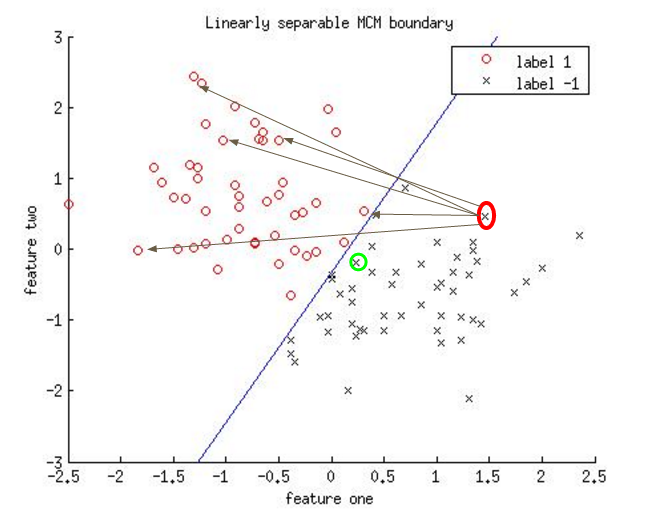
\includegraphics[scale=0.5]{scoreCalculation} 
\caption{Calculation Fuzzy Rough score}
\label{fig:frScore}
\end{center}
\end{figure}

\section{Fuzzy rough set based MCM}
Suppose $\{(x_1 , y_1 ),..., (x_M , y_M )\}$ is the training set and there are two classes A and B .We compute $s_i$ for all $x_i\epsilon A$ by equation \ref{frScoreEqn} where u are all those points who belong to class B. $s_i$ shows the degree of $x_i$ at which it belongs to A relative to the
conditional attributes. When we take $s_i$ into account for every $x_i$ , the optimal hyperplane problem is then reformulated as equation \ref{eqn:frmcm1}-\ref{eqn:frmcm4}

\begin{equation}\label{eqn:frmcm1}
min_{h,b,w,q}\:\: h + C\sum_i{s_i q_i}
\end{equation}
\begin{equation}\label{mceqn:frmcm2}
h \leq y_i(w^Tx_i+b)+ q_i \:\:\forall i={1, 2, .. M}
\end{equation}
\begin{equation}\label{eqn:frmcm3}
y_i(w^Tx_i +b) + q_i \geq s_i \:\:\forall i={1,2,.. M}
\end{equation}
\begin{equation}\label{eqn:frmcm4}
q_i \geq 0 \:\:\forall i={1, 2, ... M}
\end{equation}

continue from here.......
write about the prediction process and the working of FRMCM

\section{Where FRMCM outperforms other MCM}
TODO

\chapter{Generalization of MCM}

TODO
\section{Primal form of Generalized MCM }
\begin{equation}\label{mcmeq1}
min_{h,b,w,q,\eta}\:\: h + C_1\sum_i{q_i} + C_2\sum_i{\eta_i}
\end{equation}
\begin{equation}\label{mcmeq2}
h + \eta_i \geq y_i(w^Tx_i+b) \:\:\forall i={1, 2, .. M}
\end{equation}
\begin{equation}\label{mcmeq3}
y_i(w^Tx_i +b) + q_i \geq 1 \:\:\forall i={1,2,.. M}
\end{equation}
\begin{equation}\label{mcmeq4}
q_i \geq 0 \:\:\forall i={1, 2, ... M}
\end{equation}
\begin{equation}
\eta_i \geq 0 \:\:\forall i={1, 2, ... M}
\end{equation}

% \begin{equation}
    
% \end{equation}

\subsection{complexity analysis}
TODO
\section{Dual form of Generalized of MCM}
\subsection{Formulation of dual form}
\begin{equation}\label{mcmeq1}
min_{h,b,w,q,\eta}\:\: h + C_1\sum_i{q_i} + C_2\sum_i{\eta_i}
\end{equation}
\begin{equation}\label{mcmeq2}
h + \eta_i \geq y_i(w^Tx_i+b) \:\:\forall i={1, 2, .. M}
\end{equation}
\begin{equation}\label{mcmeq3}
y_i(w^Tx_i +b) + q_i \geq 1 \:\:\forall i={1,2,.. M}
\end{equation}
\begin{equation}\label{mcmeq4}
q_i \geq 0 \:\:\forall i={1, 2, ... M}
\end{equation}
\begin{equation}
\eta_i \geq 0 \:\:\forall i={1, 2, ... M}
\end{equation}

\begin{equation}\label{mcmeq1}
min_{h,b,w,q,\eta}\:\: h + C_1\sum_i{q_i} + C_2\sum_i{\eta_i}
\end{equation}
\begin{equation}\label{mcmeq2}
y_i(w^Tx_i+b) - h - \eta_i \leq 0 \:\:\forall i={1, 2, .. M}
\end{equation}
\begin{equation}\label{mcmeq3}
1 - y_i(w^Tx_i +b) - q_i \leq 0  \:\:\forall i={1,2,.. M}
\end{equation}
\begin{equation}\label{mcmeq4}
-q_i \leq 0 \:\:\forall i={1, 2, ... M}
\end{equation}
\begin{equation}
-\eta_i \leq 0 \:\:\forall i={1, 2, ... M}
\end{equation}
the Lagrangian equation of [ref to above equation]
\begin{equation}
\begin{split}
L=h + C_1\sum_i{q_i} + C_2\sum_i{\eta_i} + \sum_i{\alpha_i (y_i(w^Tx_i+b) - h - \eta_i)} \\
+ \sum_i{\beta_i (1 - y_i(w^Tx_i +b) - q_i)} - \sum_i{\gamma_iq_i} - \sum_i{\theta_i\eta_i}
\end{split}
\end{equation}
\begin{equation}
\frac{\partial L}{\partial h} = 1 - \sum_i{\alpha_i}
\end{equation}
\begin{equation}
\frac{\partial L}{\partial w} = \sum_i{\alpha_iy_ix_i} - \sum_i{\beta_iy_ix_i}
\end{equation}
\begin{equation}
\frac{\partial L}{\partial b} = \sum_i{\alpha_iy_i} - \sum_i{\beta_iy_i}
\end{equation}
\begin{equation}
\frac{\partial L}{\partial q_i} = C_1 - \beta_i - \gamma_i
\end{equation}
\begin{equation}
\frac{\partial L}{\partial \eta_i} = C_2 - \alpha_i -\theta_i
\end{equation}
equating all partial derivative to zero, we get
\begin{equation}
\sum_i{\alpha_i} = 1
\end{equation}
\begin{equation}
\sum_i{\alpha_iy_ix_i} - \sum_i{\beta_iy_ix_i} = 0
\end{equation}
\begin{equation}
\sum_i{\alpha_iy_i} - \sum_i{\beta_iy_i} = 0
\end{equation}
\begin{equation}
\beta_i + \gamma_i = C_1 \implies \beta_i \leq C_1
\end{equation}
\begin{equation}
\alpha_i +\theta_i = C_2 \implies \alpha_i \leq C_2
\end{equation}
\end{equation}
putting values in [ref to lag eqn]
\begin{equation}
\begin{split}
L=h(1-\sum_i\alpha_i) + \sum_i{(C_1 - \beta_i - \gamma_i)q_i} + \sum_i{(C_2 - \alpha_i - \theta_i)\eta_i} +\\ \sum_i{(\alpha_i-beta_i)y_ix_iw^T} + \sum_i{\beta_i} + \sum_i{(\alpha_i - \beta_i)y_ib}
\end{split}
\end{equation}
\begin{equation}
\begin{split}
L= \sum_i{\beta_i}
\end{split}
\end{equation}

equivalent dual problem
\begin{equation}\label{mcmeq1}
max_{\alpha,\beta}\:\: \sum_i{\beta_i}
\end{equation}
\begin{equation}\label{mcmeq4}
\sum_i{\alpha_i} = 1 \:\:\forall i={1, 2, ... M}
\end{equation}
\begin{equation}
\sum_i{\alpha_iy_ix_i} - \sum_i{\beta_iy_ix_i} = 0
\end{equation}
\begin{equation}
\sum_i{\alpha_iy_i} - \sum_i{\beta_iy_i} = 0
\end{equation}
\begin{equation}\label{mcmeq2}
0 \leq \beta_i \leq C_1
\end{equation}
\begin{equation}\label{mcmeq3}
0 \leq \alpha_i \leq C_2
\end{equation}
\subsection{complexity analysis}

\usepackage{bbm}
\chapter{Regularized MCM}

\section{Primal form of Regularized MCM}
\begin{equation}\label{mcmeq1}
min_{h,b,w,q,\eta}\:\: \frac{1}{2}||w||^2 + h + C_1\sum_i{q_i} + C_2\sum_i{\eta_i}
\end{equation}
\begin{equation}\label{mcmeq2}
h + \eta_i \geq y_i(w^Tx_i+b) \:\:\forall i={1, 2, .. M}
\end{equation}
\begin{equation}\label{mcmeq3}
y_i(w^Tx_i +b) + q_i \geq 1 \:\:\forall i={1,2,.. M}
\end{equation}
\begin{equation}\label{mcmeq4}
q_i \geq 0 \:\:\forall i={1, 2, ... M}
\end{equation}
\begin{equation}
\eta_i \geq 0 \:\:\forall i={1, 2, ... M}
\end{equation}

\subsection{complexity analysis}
\subsection{Results}


\section{Formulation of dual form}
\begin{equation}\label{mcmeq1}
min_{h,b,w,q,\eta}\:\: \frac{1}{2}||w||^2 + h + C_1\sum_i{q_i} + C_2\sum_i{\eta_i}
\end{equation}
\begin{equation}\label{mcmeq2}
h + \eta_i \geq y_i(w^Tx_i+b) \:\:\forall i={1, 2, .. M}
\end{equation}
\begin{equation}\label{mcmeq3}
y_i(w^Tx_i +b) + q_i \geq 1 \:\:\forall i={1,2,.. M}
\end{equation}
\begin{equation}\label{mcmeq4}
q_i \geq 0 \:\:\forall i={1, 2, ... M}
\end{equation}
\begin{equation}
\eta_i \geq 0 \:\:\forall i={1, 2, ... M}
\end{equation}

\begin{equation}\label{mcmeq1}
min_{h,b,w,q,\eta}\:\: \frac{1}{2}||w||^2 + h + C_1\sum_i{q_i} + C_2\sum_i{\eta_i}
\end{equation}
\begin{equation}\label{mcmeq2}
0 \geq y_i(w^Tx_i+b) - h - \eta_i \:\:\forall i={1, 2, .. M}
\end{equation}
\begin{equation}\label{mcmeq3}
0 \geq 1 - y_i(w^Tx_i +b) - q_i \:\:\forall i={1,2,.. M}
\end{equation}
\begin{equation}\label{mcmeq4}
0 \geq -q_i \:\:\forall i={1, 2, ... M}
\end{equation}
\begin{equation}
0 \geq -\eta_i \:\:\forall i={1, 2, ... M}
\end{equation}

the Lagrangian equation of [ref to above equation]
\begin{equation}
\begin{split}
L = \frac{1}{2}||w||^2 + h + C_1\sum_i{q_i} + C_2\sum_i{\eta_i} + \sum_i{\alpha_i (y_i(w^Tx_i+b) - h - \eta_i)} \\
+ \sum_i{\beta_i (1 - y_i(w^Tx_i +b) - q_i)} - \sum_i{\gamma_iq_i} - \sum_i{\theta_i\eta_i}
\end{split}
\end{equation}
\begin{equation}
\frac{\partial L}{\partial h} = 1 - \sum_i{\alpha_i}
\end{equation}
\begin{equation}
\frac{\partial L}{\partial w} = w + \sum_i{\alpha_iy_ix_i} - \sum_i{\beta_iy_ix_i}
\end{equation}
\begin{equation}
\frac{\partial L}{\partial b} = \sum_i{\alpha_iy_i} - \sum_i{\beta_iy_i}
\end{equation}
\begin{equation}
\frac{\partial L}{\partial q_i} = C_1 - \beta_i - \gamma_i
\end{equation}
\begin{equation}
\frac{\partial L}{\partial \eta_i} = C_2 - \alpha_i -\theta_i
\end{equation}
equating all partial derivative to zero, we get
\begin{equation}
\sum_i{\alpha_i} = 1
\end{equation}
\begin{equation}
w = \sum_i{(\beta_i -\alpha_i)y_ix_i}
\end{equation}
\begin{equation}
\sum_i{\alpha_iy_i} - \sum_i{\beta_iy_i} = 0
\end{equation}
\begin{equation}
\beta_i + \gamma_i = C_1 \implies \beta_i \leq C_1
\end{equation}
\begin{equation}
\alpha_i +\theta_i = C_2 \implies \alpha_i \leq C_2
\end{equation}
putting values in [ref to lag eqn]
\begin{equation}
\begin{split}
L=h(1-\sum_i\alpha_i) + \sum_i{(C_1 - \beta_i - \gamma_i)q_i} + \sum_i{(C_2 - \alpha_i - \theta_i)\eta_i} +\\ \sum_i{(\alpha_i-\beta_i)y_ix_iw^T} + \frac{1}{2}ww^T + \sum_i{\beta_i} + \sum_i{(\alpha_i - \beta_i)y_ib}
\end{split}
\end{equation}
\begin{equation}
\begin{split}
L= \sum_i{\beta_i} - \frac{1}{2}(\beta - \alpha)Q(\beta - \alpha)^T
\end{split}
\end{equation}
where
\begin{equation}
Q_{ij} = y_iy_j<x_i,x_j>
\end{equation}

equivalent dual problem
\begin{equation}\label{mcmeq1}
max_{\alpha,\beta}\:\: \sum_i{\beta_i} -  \frac{1}{2}(\beta - \alpha)Q(\beta - \alpha)^T
\end{equation}
\begin{equation}\label{mcmeq4}
\sum_i{\alpha_i} = 1 \:\:\forall i={1, 2, ... M}
\end{equation}
\begin{equation}
\sum_i{\alpha_iy_i} - \sum_i{\beta_iy_i} = 0
\end{equation}
\begin{equation}\label{mcmeq2}
0 \leq \beta_i \leq C_1
\end{equation}
\begin{equation}\label{mcmeq3}
0 \leq \alpha_i \leq C_2
\end{equation}

which is equivalent to
\begin{equation}\label{mcmeq1}
min_{\alpha,\beta}\:\: \frac{1}{2}(\beta - \alpha)Q(\beta - \alpha)^T - \sum_i{\beta_i}
\end{equation}
\begin{equation}\label{mcmeq4}
\sum_i{\alpha_i} = 1 \:\:\forall i={1, 2, ... M}
\end{equation}
\begin{equation}
\sum_i{\alpha_iy_i} - \sum_i{\beta_iy_i} = 0
\end{equation}
\begin{equation}\label{mcmeq2}
0 \leq \beta_i \leq C_1
\end{equation}
\begin{equation}\label{mcmeq3}
0 \leq \alpha_i \leq C_2
\end{equation}


if we assume $\delta_i = \beta_i - \alpha_i$, then we can say $w = \sum_i{\deta_iy_ix_i}$ and the objective dual problem becomes as following eqn[REF]
\begin{equation}\label{mcmeq1}
min_{\alpha,\beta}\:\: \frac{1}{2}\delta Q \delta^T - \sum_i{\delta_i} +\sum_i{\alpha_i}
\end{equation}
\begin{equation}\label{mcmeq4}
\sum_i{\alpha_i} = 1 \:\:\forall i={1, 2, ... M}
\end{equation}
\begin{equation}
\sum_i{\delta_iy_i} = 0
\end{equation}
\begin{equation}\label{mcmeq2}
0 \leq \delta_i + \alpha_i \leq C_1
\end{equation}
\begin{equation}\label{mcmeq3}
0 \leq \alpha_i \leq C_2
\end{equation}

this implementation was 50\% faster

\subsection{complexity analysis}
\subsection{Results}
\section{Dual Coordinate Descent for large scale MCM}
if we assume $x_i = \{x_i,1\}$ and w = $\{w ,b\}$
the the dual form becomes
\begin{equation}\label{mcmeq1}
min_{\alpha,\beta}\:\: \frac{1}{2}(\beta - \alpha)Q(\beta - \alpha)^T - \sum_i{\beta_i}
\end{equation}
\begin{equation}\label{mcmeq4}
\sum_i{\alpha_i} = 1 \:\:\forall i={1, 2, ... M}
\end{equation}
\begin{equation}\label{mcmeq2}
0 \leq \beta_i \leq C_1
\end{equation}
\begin{equation}\label{mcmeq3}
0 \leq \alpha_i \leq C_2
\end{equation}

In above case we have considered l1-loss function. In more general form i.e. when considering l2-loss the equations comes out to be....

\begin{equation}\label{mcmeq1}
min_{\alpha,\beta} \:\: \frac{1}{2}(\beta - \alpha)Q(\beta - \alpha)^T - \sum_i{\beta_i} + \frac{1}{4C_1}\sum_i{\beta_i^2} + \frac{1}{4C_2}\sum_i{\alpha_i^2}
\end{equation}
\begin{equation}\label{mcmeq4}
\sum_i{\alpha_i} = 1 \:\:\forall i={1, 2, ... M}
\end{equation}
\begin{equation}\label{mcmeq2}
0 \leq \beta_i \leq C_1
\end{equation}
\begin{equation}\label{mcmeq3}
0 \leq \alpha_i \leq C_2
\end{equation}
for the ease of calculation we assume $C_1 = C_2 = C$.\\
By using the concept of sub-lagrangian form, we can convert the above problem into a simpler one as below [REF TO BE GIVEN]
\begin{equation}\label{mcmeq1}
min_{\alpha,\beta} \:\: \frac{1}{2}(\beta - \alpha)Q(\beta - \alpha)^T - \sum_i{\beta_i} + \frac{1}{4C}\sum_i{\beta_i^2} + \frac{1}{4C}\sum_i{\alpha_i^2} + \lambda(\sum_i\alpha_i -1)
\end{equation}
\begin{equation}\label{mcmeq2}
0 \leq \beta_i \leq C_1
\end{equation}
\begin{equation}\label{mcmeq3}
0 \leq \alpha_i \leq C_2
\end{equation}

let's say equation 1 of above [REF] is a function $f$
\begin{equation}\label{mcmeq1}
f = \frac{1}{2}(\beta - \alpha)Q(\beta - \alpha)^T - \sum_i{\beta_i} + \frac{1}{4C}\sum_i{\beta_i^2 + \alpha_i^2} + \lambda(\sum_i\alpha_i -1)
\end{equation}

\begin{equation}\label{mcmeq1}
f = \frac{1}{2}(\beta - \alpha)Q(\beta - \alpha)^T - \mathbbm{1}\beta + \frac{1}{4C}{\beta\beta^T + \alpha\alpha^T}  + \lambda ( \mathbbm{1}\alpha - 1)
\end{equation}

Gradient of f with respect to $\alpha$ and $\beta$ can be calculated by following [REF]
\begin{equation}
G_\beta = Q(\beta - \alpha) -1 + \frac{1}{2C}\beta
\end{equation}
\begin{equation}
G_\alpha = \lambda - G_\beta -1 + \frac{1}{2C}(\beta + \alpha)
\end{equation}

let's say $d = \frac{1}{2C}$ for l2-loss function and  $d = 0$ for l1-loss function then the generic form of gradient will be following[REF]
\begin{equation}
G_\beta = Q(\beta - \alpha) -1 + d\beta
\end{equation}
\begin{equation}
G_\alpha = \lambda - G_\beta -1 + d(\beta + \alpha)
\end{equation}

the 2nd order gradient will be Q+d

So the DCD for large scale MCM will be ass following [REF]

\begin{algorithm}
\caption{Dual Coordinate Descent}\label{array-sum}
\begin{algorithmic}[1]
	\Procedure{dcd}{}
	\State Initialize all $\alpha_i$ to 1/M and $\beta_i$ to 0 and calculate w, $w_j \gets \sum_i{(\beta_i-\alpha_i)y_ix_ij}$
	\While {Not converged}
    	\For {each example $i$ in A }
		    \State Gradients $G\alpha = y_ix_iw_i - 1 + d\beta_i \:and\:G\alpha = \lambda - G\beta - 1 + d(\beta_i+\alpha_i)$
		    \State $PG_\alpha \gets 0, PG_\beta \gets 0$
		    \If {$\alpha_i = 0$}
		    \State $PG_\alpha = min(G_\alpha,0)$
		    \ElsIf {$\alpha_i = C_2$}
		    \State $PG_\alpha = max(G_\alpha,0)$
		    \Else
		    \State $PG_\alpha = G_\alpha$
		    \EndIf
		    \If {$\beta_i = 0$}
		    \State $PG_\beta = min(G_\beta,0)$
		    \ElsIf {$\beta_i = C_1$}
		    \State $PG_\beta = max(G_\beta,0)$
		    \Else
		    \State $PG_\beta = G_\beta$
		    \EndIf
            \State $\delta_\alpha \gets 0 , \delta_\beta \gets 0$
            \If{$|PG\alpha| \neq 0$}
                \State $\alpha_{old} = \alpha_i$
                \State $\alpha_i \gets min(max((\alpha_i - G_\alpha/\overline{Q}_{ii}),0),C_2)$
                \State $\delta_\alpha = y_i(\alpha_i - \alpha_{old})$
            \EndIf
            \If{$|PG\beta| \neq 0$}
                \State $\beta_{old} = \beta_i$
                \State $\beta_i \gets min(max((\beta_i - G_\beta/\overline{Q}_{ii}),0),C_1)$
                \State $\delta_\beta = y_i(\beta_i - \beta_{old})$
            \EndIf
            \If{$|PG\alpha| \neq 0$ OR $|PG\beta| \neq 0$}
                \State $w \gets  w + (\delta_\beta-\delta_\alpha)y_ix_i$
            \EndIf      
    	\EndFor
	\EndWhile
	\EndProcedure
\end{algorithmic}
\end{algorithm}


\begin{algorithm}
\caption{DCD with shrinking}\label{array-sum}
\begin{algorithmic}[1]
	\Procedure{dcd}{}
	\State Initialize all $\alpha_i$ to 1/M and $\beta_i$ to 0 and calculate w, $w_j \gets \sum_i{(\beta_i-\alpha_i)y_ix_ij}$
	\State $G_{\alpha old} \gets -\infty$ , $G_{\beta old} \gets -\infty$ 
	\State $\overline{G}_{\alpha new} \gets \infty , \overline{G}_{\beta old} \gets \infty$
	\State A $\gets {1..M}$
	\While {Not converged}
    	\State $G{_\alpha new} \gets \infty$ , $G{_\beta new} \gets \infty$ 
	    \State $\overline{G}_{\alpha new} \gets -\infty , \overline{G}_{\beta new} \gets -\infty$
    	\For {each example $i$ in A }
		    \State Gradients $G\alpha = y_ix_iw_i - 1 + d\beta_i \:and\:G\alpha = \lambda - G\beta - 1 + d(\beta_i+\alpha_i)$
		    \State $PG_\alpha \gets 0, PG_\beta \gets 0$
		    \If {$\alpha_i = 0$}
		    \State Remove $i$ from $A\: if\: G_\alpha > \overline{G}_{\alpha old}$
		    \State $PG_\alpha = G_\alpha\:if\: G_\alpha < 0$
		    \ElsIf {$\alpha_i = C_2$}
		    \State Remove $i$ from $A\: if\: G_\alpha < G_{\alpha old}$
		    \State $PG_\alpha \gets G_\alpha\:if\: G_\alpha > 0$
		    \Else
		    \State $PG_\alpha \gets G_\alpha$
		    \EndIf
		    \State $\overline{G}_{\alpha new}\gets max(PG_\alpha,\overline{G}_{\alpha new})\:,\: 
                G_{\alpha new}\gets min(PG_\alpha,G_{\alpha new})$
            \If {$\beta_i = 0$}
		    \State Remove $i$ from $A\: if\: G_\beta > \overline{G}_{\beta old}$
		    \State $PG_\beta = G_\beta\:if\: G_\beta < 0$
		    \ElsIf {$\beta_i = C_1$}
		    \State Remove $i$ from $A\: if\: G_\beta < G_{\beta old}$
		    \State $PG_\beta \gets G_\beta\:if\: G_\beta > 0$
		    \Else
		    \State $PG_\beta \gets G_\beta$
		    \EndIf
		    \State $\overline{G}_{\beta new}\gets max(PG_\beta,\overline{G}_{\beta new})\:,\: 
                G_{\beta new}\gets min(PG_\beta,G_{\beta new})$
            \State $\delta_\alpha \gets 0 , \delta_\beta \gets 0$
            \If{$|PG\alpha| \neq 0$}
                \State $\alpha_{old} = \alpha_i$
                \State $\alpha_i \gets min(max((\alpha_i - G_\alpha/\overline{Q}_{ii}),0),C_2)$
                \State $\delta_\alpha = y_i(\alpha_i - \alpha_{old})$
            \EndIf
            \algstore{myalg}
        \end{algorithmic}
\end{algorithm}
\begin{algorithm}
\begin{algorithmic}
\algrestore{myalg}
            \If{$|PG\beta| \neq 0$}
                \State $\beta_{old} = \beta_i$
                \State $\beta_i \gets min(max((\beta_i - G_\beta/\overline{Q}_{ii}),0),C_1)$
                \State $\delta_\beta = y_i(\beta_i - \beta_{old})$
            \EndIf
            \If{$|PG\alpha| \neq 0$ OR $|PG\beta| \neq 0$}
                \State $w \gets  w + (\delta_\beta-\delta_\alpha)y_ix_i$
            \EndIf      
    	\EndFor
        \If{$\overline{G}_{\alpha new} - G_{\alpha new} \leq \epsilon$ AND $\overline{G}_{\beta new} - G_{\beta new} \leq \epsilon$}
        \If{ $A = \{1,..M\} $}
        \State BREAK
        \Else
        \State $A \gets \{1,..M\}$
        \State $\overline{G}_{\alpha old} \gets \infty , G_{\alpha old} \gets -\infty
        \overline{G}_{\beta old} \gets \infty , G_{\beta old} \gets -\infty$
        \EndIf
        \EndIf
        \State if $\overline{G}_{\alpha old} \leq 0 \:then\: \overline{G}_{\alpha old} \gets \infty \:else\: \overline{G}_{\alpha old} \gets \overline{G}_{\alpha new}$
    	\State if $G_{\alpha old} \geq 0 \:then\: G_{\alpha old} \gets -\infty \:else\: G_{\alpha old} \gets G_{\alpha new}$
    	\State if $\overline{G}_{\beta old} \leq 0 \:then\: \overline{G}_{\beta old} \gets \infty \:else\: \overline{G}_{\beta old} \gets \overline{G}_{\beta new}$
    	\State if $G_{\beta old} \geq 0 \:then\: G_{\beta old} \gets -\infty \:else\: G_{\beta old} \gets G_{\beta new}$
	\EndWhile
	\EndProcedure
\end{algorithmic}
\end{algorithm}


\subsection{complexity analysis}
\subsection{Results}
%Replace \lipsum with text.
% You may have as many sections as you please. This is just for reference.

\section{Comparison of Fuzzy Rough MCM with other models}


\section{Comparison of improved MCM with other models}


% Please add the following required packages to your document preamble:
% \usepackage{booktabs}
% \usepackage{graphicx}
\begin{table}[]
\centering
\resizebox{\textwidth}{!}{%
\begin{tabular}{@{}lllllllll@{}}
\toprule
\textbf{Data-set} & \textbf{MCM (primal)} & \textbf{MCM (RBF)} & \textbf{MCM (dual)} & \textbf{Reg MCM(DCD)} & \textbf{DCD+RBF} & \textbf{SVM linear} & \textbf{SVM(RBF)} & \textbf{Liblinear} \\ \midrule
iono-sphere & 92.5373 & 67.1642 & 92.5373 & 89.5522 & 89.5522 & 89.5522 & 65.6716 & 89.55\% \\
sonar & 77.5 & 60 & 77.5 & 90 & 90 & 85 & 60 & 77.50\% \\
blogger & 75 & 85 & 75 & 65 & 85 & 65 & 65 & 80\% \\
tae & 70.3704 & 81.4815 & 74.0741 & 74.0741 & 74.0741 & 70.3704 & 70.3704 & 70.37\% \\
bupa & 62.3188 & 53.6232 & 63.7681 & 65.2174 & 69.5652 & 63.7681 & 49.2754 & 56.52\% \\
pima & 78.2895 & 67.7632 & 76.9737 & 78.2895 & 78.2895 & 78.9474 & 61.8421 & 62.50\% \\
news20b & - & - & - & 94.573 & - & 96.5241 & 50.012 & 96.60\% \\
mnist38 & - & - & - & 95.6653 & 97.6311 & 96.1694 & 98.29\% & 96.12\% \\
real-sim & - & - & - & 79.7179 & - & 97.4967 & 69.2414 & 97.63\% \\
webspam & - & - & - & 98.2738 & - & - & - & 98.41\% \\
kddb & - & - & - & 73.0125 &  & 87.3636 & 88.7725 & 87.44\% \\
Colon & 58.3333 & 91.6667 & 83.3333 & 75.00\% & 91.6667 & 66.6667 & 8.33333 & 58.33\% \\
leukemia & 57.1429 & 42.8571 & 57.1429 & 57.1429 & 42.8571 & 57.1429 & 57.1429 & 42.8571 \\
rac & 50 & 50 & 50 & 66.6667 & 33.3333 & 33.3333 & 50 & 50\% \\
raoa & 33.333 & 16.6667 & 16.6667 & 66.6667 & 50 & 33.3333 & 33.3333 & 83.33\% \\
a9a & - & - & - & 84.4297 &  & 84.9764 & 84.8167 & 84.9641 \\ \bottomrule
\end{tabular}%
}
\caption{Comparison of accuracies various data-sets' on different model}
\label{table:accuracyall}
\end{table}


% Please add the following required packages to your document preamble:
% \usepackage{booktabs}
% \usepackage{graphicx}
\begin{table}[]
\centering
\resizebox{\textwidth}{!}{%
\begin{tabular}{@{}lllllllll@{}}
\toprule
\textbf{Data-set} & \textbf{MCM (primal)} & \textbf{MCM (RBF)} & \textbf{MCM (dual)} & \textbf{Reg MCM(DCD)} & \textbf{DCD+RBF} & \textbf{SVM linear} & \textbf{SVM(RBF)} & \textbf{Liblinear} \\ \midrule
iono-sphere & 33 & 284 & 284 & 75 & 144 & 87 & 206 & 189 \\
sonar & 60 & 168 & 168 & 70 & 132 & 114 & 162 & 135 \\
bloggers & 5 & 80 & 80 & 53 & 73 & 54 & 50 & 80 \\
tae & 5 & 124 & 124 & 111 & 91 & 90 & 88 & 124 \\
bupa & 6 & 276 & 276 & 196 & 213 & 193 & 220 & 253 \\
pima & 8 & 616 & 616 & 324 & 574 & 322 & 420 & 613 \\
news20b & - & - & - & 6596 &  & 7384 & 15996 & 9764 \\
mnist38 & - & - & - & 1119 & 6589 & 947 & 1813 & 2114 \\
real-sim & - & - & - & 5488 &  & 9428 & 35580 & 13039 \\
webspam & - & - & - & 6795 & - & - & - & 7422 \\
kddb & - & - & - & 58017 &  & 59301 & 27858 & 60604 \\
Colon & 50 & 50 & 50 & 50 & 50 & 26 & 44 & 26 \\
leukemia & 58 & 58 & 56 & 58 & 58 & 53 & 58 & 55 \\
rac & 27 & 27 & 5 & 27 & 27 & 27 & 27 & 27 \\
raoa & 25 & 25 & 19 & 23 & 25 & 21 & 25 & 21 \\
a9a & - & - & - & 11858 &  & 11533 & 11958 & 19796 \\ \bottomrule
\end{tabular}%
}
\caption{Comparison of number of support vectors various data-sets' on different model}
\label{table:NSVall}
\end{table}


% Please add the following required packages to your document preamble:
% \usepackage{booktabs}
% \usepackage{graphicx}
\begin{table}[]
\centering
\resizebox{\textwidth}{!}{%
\begin{tabular}{@{}lllllllll@{}}
\toprule
\textbf{Data-set} & \textbf{MCM (primal)} & \textbf{MCM (RBF)} & \textbf{MCM (dual)} & \textbf{Reg MCM(DCD)} & \textbf{DCD+RBF} & \textbf{SVM linear} & \textbf{SVM(RBF)} & \textbf{Liblinear} \\ \midrule
iono-sphere & 6.807844 & 3.180053 & 1.371437 & 0.007441 & 2.39704 & 0.006064 & 0.001721 & 0.007267 \\
sonar & 2.103759 & 0.703101 & 0.920255 & 0.028046 & 1.72688 & 0.003896 & 0.000956 & 0.003854 \\
bloggers & 0.145067 & 0.147382 & 0.423042 & 0.000689 & 0.013181 & 0.001261 & 0.000451 & 0.000891 \\
tae & 0.234263 & 4.311576 & 0.37578 & 0.001371 & 0.056936 & 0.003007 & 0.000867 & 0.009123 \\
bupa & 0.875911 & 6.341775 & 0.868488 & 0.004054 & 0.158725 & 0.099253 & 0.001276 & 0.020284 \\
pima & 18.152894 & 33.167435 & 0.505668 & 0.003823 & 4.35 & 2.485059 & 0.005462 & 0.041092 \\
news20b & - & - &  & 7.74023 &  & 933.442098 & 648.639779 & 7.630068 \\
mnist38 & - & - &  & 3.51589 & 12270.2 & 137.758703 & 33.771507 & 17.748283 \\
real-sim & - & - &  & 0.738976 &  & 651.155052 & 1254.963437 & 13.884177 \\
webspam & - & - &  & 130.395 & - & - & - & 1568.455279 \\
kddb & - & - &  & 10.9602 &  & 5367.86111 & 601.860198 & 28.601222 \\
Colon & 0.086017 & 0.57646 & 1.49381 & 0.128049 & 0.179784 & 0.010611 & 0.009974 & 0.060945 \\
leukemia & 0.281447 & 3.621722 & 6.326389 & 1.04047 & 2.58614 & 0.088341 & 0.07027 & 0.178956 \\
rac & 0.133488 & 5.060754 & 14.624991 & 3.24957 & 16.2942 & 0.186384 & 0.196265 & 0.52741 \\
raoa & 0.05205 & 1.139824 & 4.345408 & 1.14475 & 5.29395 & 0.045654 & 0.206045 & 0.180704 \\
a9a & - & - & - & 0.465888 &  & 64.990886 & 48.368211 & 0.654848 \\ \bottomrule
\end{tabular}%
}
\caption{Comparison of training time(in Sec) of various data-sets' on different model}
\label{table:timeall}
\end{table}

\section{Kernelization of Regulaized MCM}
\subsection{complexity analysis}
\subsection{Results}
TODO

\chapter{Conclusion and Future Work}

%Replace \lipsum with text.
% You may have as many sections as you please. This is just for reference.

\section{Conclusion}

TODO

\section{Limitation}

TODO

\section{Future Work}

TODO


% \include{chapter6}

%\include{chapter7}

\bibliographystyle{plain}
\bibliography{biblio}

\appendix
\chapter{Appendix}

\section{Implementation code}
\lipsum[1]


\end{document}
	